\documentclass[11pt]{article}
\usepackage{geometry}                
\geometry{letterpaper}                   





\usepackage[english]{babel}
\usepackage[utf8x]{inputenc}
\usepackage{amsmath}
\usepackage{tikz}
\usetikzlibrary{positioning}

\usetikzlibrary{arrows,automata}


%\usepackage[latin1]{inputenc}
\usepackage{graphicx}
\usepackage{amssymb}
\usepackage{epstopdf}
\usepackage{natbib}
\usepackage{amssymb, amsmath}
\DeclareGraphicsRule{.tif}{png}{.png}{`convert #1 `dirname #1`/`basename #1 .tif`.png}
\title{Airplane Boarding}
\author{Anton Schäfer, Nils Blach}
%\date{date} 

\begin{document}



\thispagestyle{empty}

\begin{center}
\includegraphics[width=5cm]{ETHlogo.eps}

\bigskip


\bigskip


\bigskip


\LARGE{ 	Lecture with Computer Exercises:\\ }
\LARGE{ Modelling and Simulating Social Systems\\}

\bigskip

\bigskip

\small{Project Report}\\

\bigskip

\bigskip

\bigskip

\bigskip


\begin{tabular}{|c|}
\hline
\\
\textbf{\LARGE{Insert Title Here}}\\
\textbf{\LARGE{...}}\\
\\
\hline
\end{tabular}
\bigskip

\bigskip

\bigskip

\LARGE{Name 1, Name 2  \& [...]}



\bigskip

\bigskip

\bigskip

\bigskip

\bigskip

\bigskip

\bigskip

\bigskip

Zurich\\
Dec 2018\\

\end{center}



\newpage

%%%%%%%%%%%%%%%%%%%%%%%%%%%%%%%%%%%%%%%%%%%%%%%%%

\newpage
\section*{Agreement for free-download}
\bigskip


\bigskip


\large We hereby agree to make our source code for this project freely available for download from the web pages of COSS. Furthermore, we assure that all source code is written by ourselves and is not violating any copyright restrictions.

\begin{center}

\bigskip


\bigskip


\begin{tabular}{@{}p{3.3cm}@{}p{6cm}@{}@{}p{6cm}@{}}
\begin{minipage}{3cm}

\end{minipage}
&
\begin{minipage}{6cm}
	\vspace{2mm} \large Anton Sch{\"a}fer

 \vspace{\baselineskip}

\end{minipage}
&
\begin{minipage}{6cm}

\large Nils Blach

\end{minipage}
\end{tabular}


\end{center}
\newpage

%%%%%%%%%%%%%%%%%%%%%%%%%%%%%%%%%%%%%%%



% IMPORTANT
% you MUST include the ETH declaration of originality here; it is available for download on the course website or at http://www.ethz.ch/faculty/exams/plagiarism/index_EN; it can be printed as pdf and should be filled out in handwriting


%%%%%%%%%% Table of content %%%%%%%%%%%%%%%%%

\tableofcontents

\newpage

%%%%%%%%%%%%%%%%%%%%%%%%%%%%%%%%%%%%%%%



\section{Abstract}

\section{Individual contributions}
\paragraph{Model:} Both
\paragraph{Data Collection/Calculation:} Anton Sch{\"a}fer
\paragraph{Data Display/Graphs:} Nils Blach
\paragraph{Paper:} Both

\section{Introduction and Motivations}

\section{Description of the Model}

\subsection{Overview}

Our model realistically simulates the process of airplane boarding. It aims to provide reasonable information about how long it takes until all people are seated and how long it takes until a specific person is seated, depending on different boarding methods, luggage loads, and passenger count.  In order to achieve this, it focuses on actions taking place in the aisle, such as passengers moving, passengers storing items, and passengers moving into their seat.


\subsection{The Boarding Process}
\paragraph{At the gate}
Before boarding, passengers usually wait at the gate. When boarding is announced, they start to line up either in random order, or by group, depending on the airline or flight. Commonly used grouping schemes are either by blocks of seats, or by letter (A,B,...,F). The boarding agent announces which group is next to board the plane, so the passengers will enter the plane in the order of their assigned groups. Still, the order in which passengers from the same block enter the plane is random. 

\paragraph{Entering the plane}
Passengers get to the plane via bus or through a jet bridge and enter the plane through either the front door or back door (or some middle door, if the airplane is big), or through both doors. Once inside the plane, passengers usually first try to find their seat.  Before sitting down, however, they may need to store their hand luggage. 
\paragraph{Hand luggage} The three main types of hand luggage passengers carry are purses, backpacks and suitcases. Purses and some backpacks are usually stored under the seat in front, while suitcases and other backpacks need to be put in the overead compartments. When searching for an overhead compartment to store their items, passengers generally first check, if there space in a compartment right above their seat. When they see that it is full already, they usually store their luggage in the next free compartment they see. However, passengers usually avoid walking back into the direction they came from, as this would mean going against the flow of passengers in the narrow aisle.

\paragraph{Entering seat} After storing all their big hand luggage, passengers walk to their row in order to sit down. If noone sits inbetween them and their seat, they can sit down. Otherwise, the sitting passengers first have to get out of the row, in order to let in the arriving passenger.
\\\\
Once all passengers are seated, boarding is completed.

\subsection{Our model}

We want to gain insight on the efficiency of various boarding methods, and the impact of luggage load and passenger count on the time it takes individuals and all passengers to board a plane. Thus, what happens in the plane is crucial, while what is taking place in the airport, jet bridge, and bus barely have significant effects on the boarding time, other than determining the order in which people arrive at the plane door. We therefore decided to only model the events taking place inside the airplane. In order to still take into account the impact of different boarding strategies chosen by the gate agent, we assume the passengers all enter the plane in a certain order given by their seats. We will call such an order (of seats/passengers by seat) a boarding sequence.
Although we have to keep track of which passengers are already sitting, it is not relvevant what the sitting passengers are doing. Hence, for our model, we focus only on what is happening in the aisle and discard most other irrelevant parts of the plane.

We only consider airplanes with one door at the front, as all other airplanes with $n \geq 2$ doors can be divided in $n$ sections with one door. Then, boarding can simultaneously be modeled in each section individually, yielding the same result, if one assumes, that in reality, passengers entering the plane in one section will never go to a different section.
When choosing reasonable sections and assuming passengers behave rational, this can indeed be guaranteed. Similarly, we only consider airplanes with one aisle, as all other planes can again be divided into sections with one aisle each. Additionally, the plane used for modelling is configureable. Thus, our model applies to almost all airplanes (when dividing them in sections if necessary).

We use an actor based model, where the actors are passengers. For simplicity, we divide the continuous time interval in discrete timesteps. The actors move around in the aisle, which is a one dimensional line divided in discrete space units. Two actors can never be at the same position in the aisle, unless they are moving in opposite directions and have to pass each other. Then, they can switch positions. We model the boarding process of an actor as follows:

\paragraph{Entering the plane}
An actor enters the plane as soon as all actors that he is behind of in the boarding sequence  have entered the plane and if there is enough free space in the aisle for a new actor to enter. The actor then appears at the very start of the aisle.




\paragraph{Hand luggage}
For each actor, we only consider the pieces of luggage they need to store in an overhead compartment. We discard their other luggage, as it will be stored underneath the front seat, and thus has a negligible impact on boarding time. Also, instead of taking into account every single overhead compartment, for any pair of opposite compartments, our model uses one single compartment that holds twice as many items, and covers the same space of the aisle. This simplification is realistic, as from each position in the aisle, passengers can reach the compartments on both sides. Because of this abstraction, in the remainder of this paper, when referring to a "compartment" while speaking about our model, we mean one single big compartment corresponding to two opposite actual compartments.

	As soon as an actors can see their seat, they determine if they can store all their luggage in the comparment above their seat. If they can, they will store their luggage there, otherwise, they will store as much of their luggage as possible in the next free compartments they see. However, at first, they only move forward in order not to go against the flow. Only when they arrive at the very end of the plane and can still not store their luggage, they search for a free compartment towards the front of the plane.


\paragraph{Entering seat}
After storing all their luggage, the actors go to their seat in order to sit down. If other sitting passengers are obstructing the way to their seat, these passengers need to move out of their seat first in order to let in the arriving actor. The arriving actor blocks the aisle during this whole time.
\\\\
Boarding is completed as soon as every actor entered their seat.


\subsection{Our Model vs. Van Landeghem's and Beuselinck's Model} 







\section{Implementation}
\begin{figure}[h!]
	\center
\begin{tabular}{|ll|l|}
	\hline
	State & &Description\\
	\hline
0 &     & not yet in plane                        \\
\hline
1 & 1/0 & looking for storage room by seat        \\
  & 1/1 & looking for storage room behind seat    \\
  & 1/2 & looking for storage room further front  \\
  \hline
2 & 2/0 & storing luggage (coming from state 1/0) \\
  & 2/1 & storing luggage (coming from state 1/1) \\
  & 2/2 & storing luggage (coming from state 1/2) \\
  \hline
3 &     & going to seat                           \\
\hline
4 &     & sitting down                            \\
\hline
5 &     & sitting in seat       \\                 
\hline

\end{tabular}
\caption{States an actor can be in}
\label{tab:states}
\end{figure}

\begin{figure}[h!]

	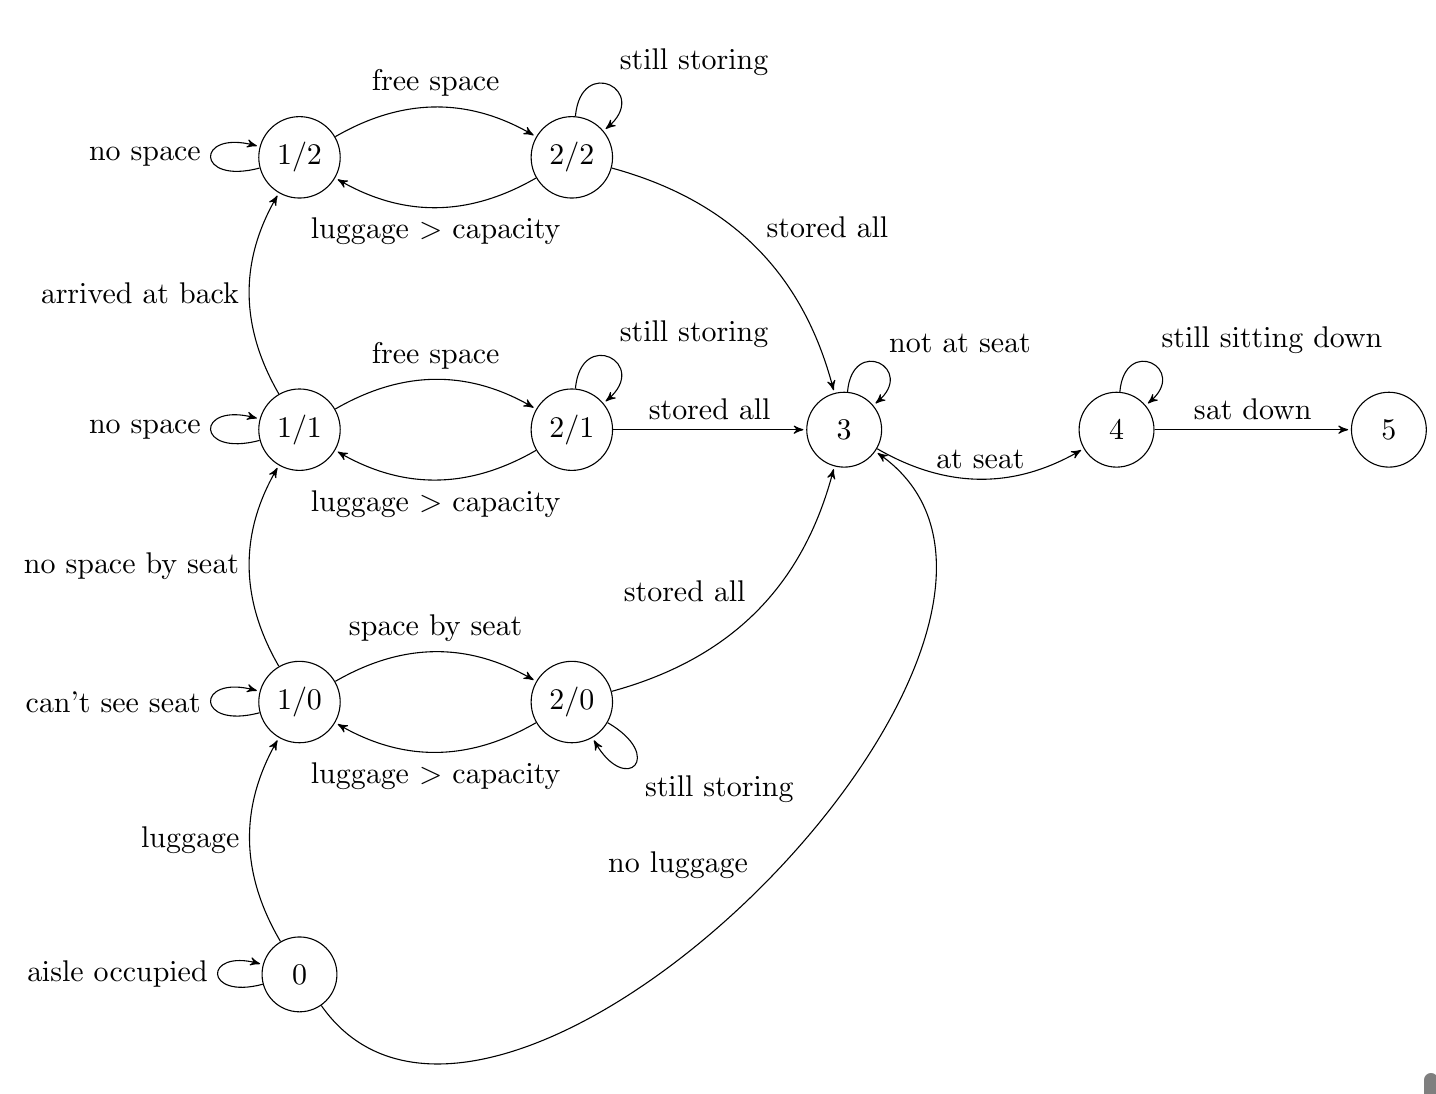
\includegraphics[width=\linewidth]{images/fsm.png}
	\label{fig:fsm}
	\caption{Finite state machine describing the states an actor can be in.}
%\begin{tikzpicture}[->,>=stealth',shorten >=1pt,auto,node distance=3.5cm,
%        scale = 1,transform shape]

%\node[state] (0) [] {$0$};
% \node[state] (1/0) [above of=0] {$1/0$};
% \node[state] (1/1) [above of=1/0] {$1/1$};
% \node[state] (1/2) [above of=1/1] {$1/2$};
% \node[state] (2/0) [right of=1/0] {$2/0$};
% \node[state] (2/1) [right of=1/1] {$2/1$};
% \node[state] (2/2) [right of=1/2] {$2/2$};
% \node[state] (3) [right of=2/1] {$3$};
% \node[state] (4) [right of=3] {$4$};
% \node[state] (5) [right of=4] {$5$};
%
% \path (0) edge   [bend left]           node {luggage} (1/0)
%       (0) edge  [bend right=100]            node {no luggage} (3)
%       (0) edge  [loop left]            node {aisle occupied} (0)
%       (1/0) edge  [loop left]            node {can't see seat} (1/0)
%       (1/0) edge    [bend left]          node {no space by seat} (1/1)
%       (1/0) edge   [bend left]           node {space by seat} (2/0)
%       (1/1) edge  [loop left]            node {no space} (1/1)
%       (1/1) edge   [bend left]           node {arrived at back} (1/2)
%       (1/1) edge   [bend left]            node {free space} (2/1)
%       (1/2) edge   [loop left]           node {no space} (1/2)
%       (1/2) edge    [bend left]           node {free space} (2/2)
%       (2/0) edge     [out=330,in=300,looseness=8]        node {still storing} (2/0)
%       (2/0) edge    [bend left]          node {luggage $>$ capacity} (1/0)
%       (2/0) edge     [bend right]         node {stored all} (3)
%       (2/1) edge      [out=85,in=40,looseness=5]        node {still storing} (2/1)
%       (2/1) edge     [bend left]         node {luggage $>$ capacity} (1/1)
%       (2/1) edge              node {stored all} (3)
%       (2/2) edge     [out=85,in=40,looseness=5]         node {still storing} (2/2)
%       (2/2) edge     [bend left]         node {luggage $>$ capacity} (1/2)
%       (2/2) edge     [bend left]         node {stored all} (3)
%       (3) edge     [out=85,in=40,looseness=5]       node {not at seat} (3)
%       (3) edge     [bend right]         node {at seat} (4)
%       (4) edge      [out=85,in=40,looseness=5]         node {still sitting down} (4)
%       (4) edge              node {sat down} (5);
%
%\end{tikzpicture}
\end{figure}
 



\section{Simulation Results and Discussion}
\begin{figure}
	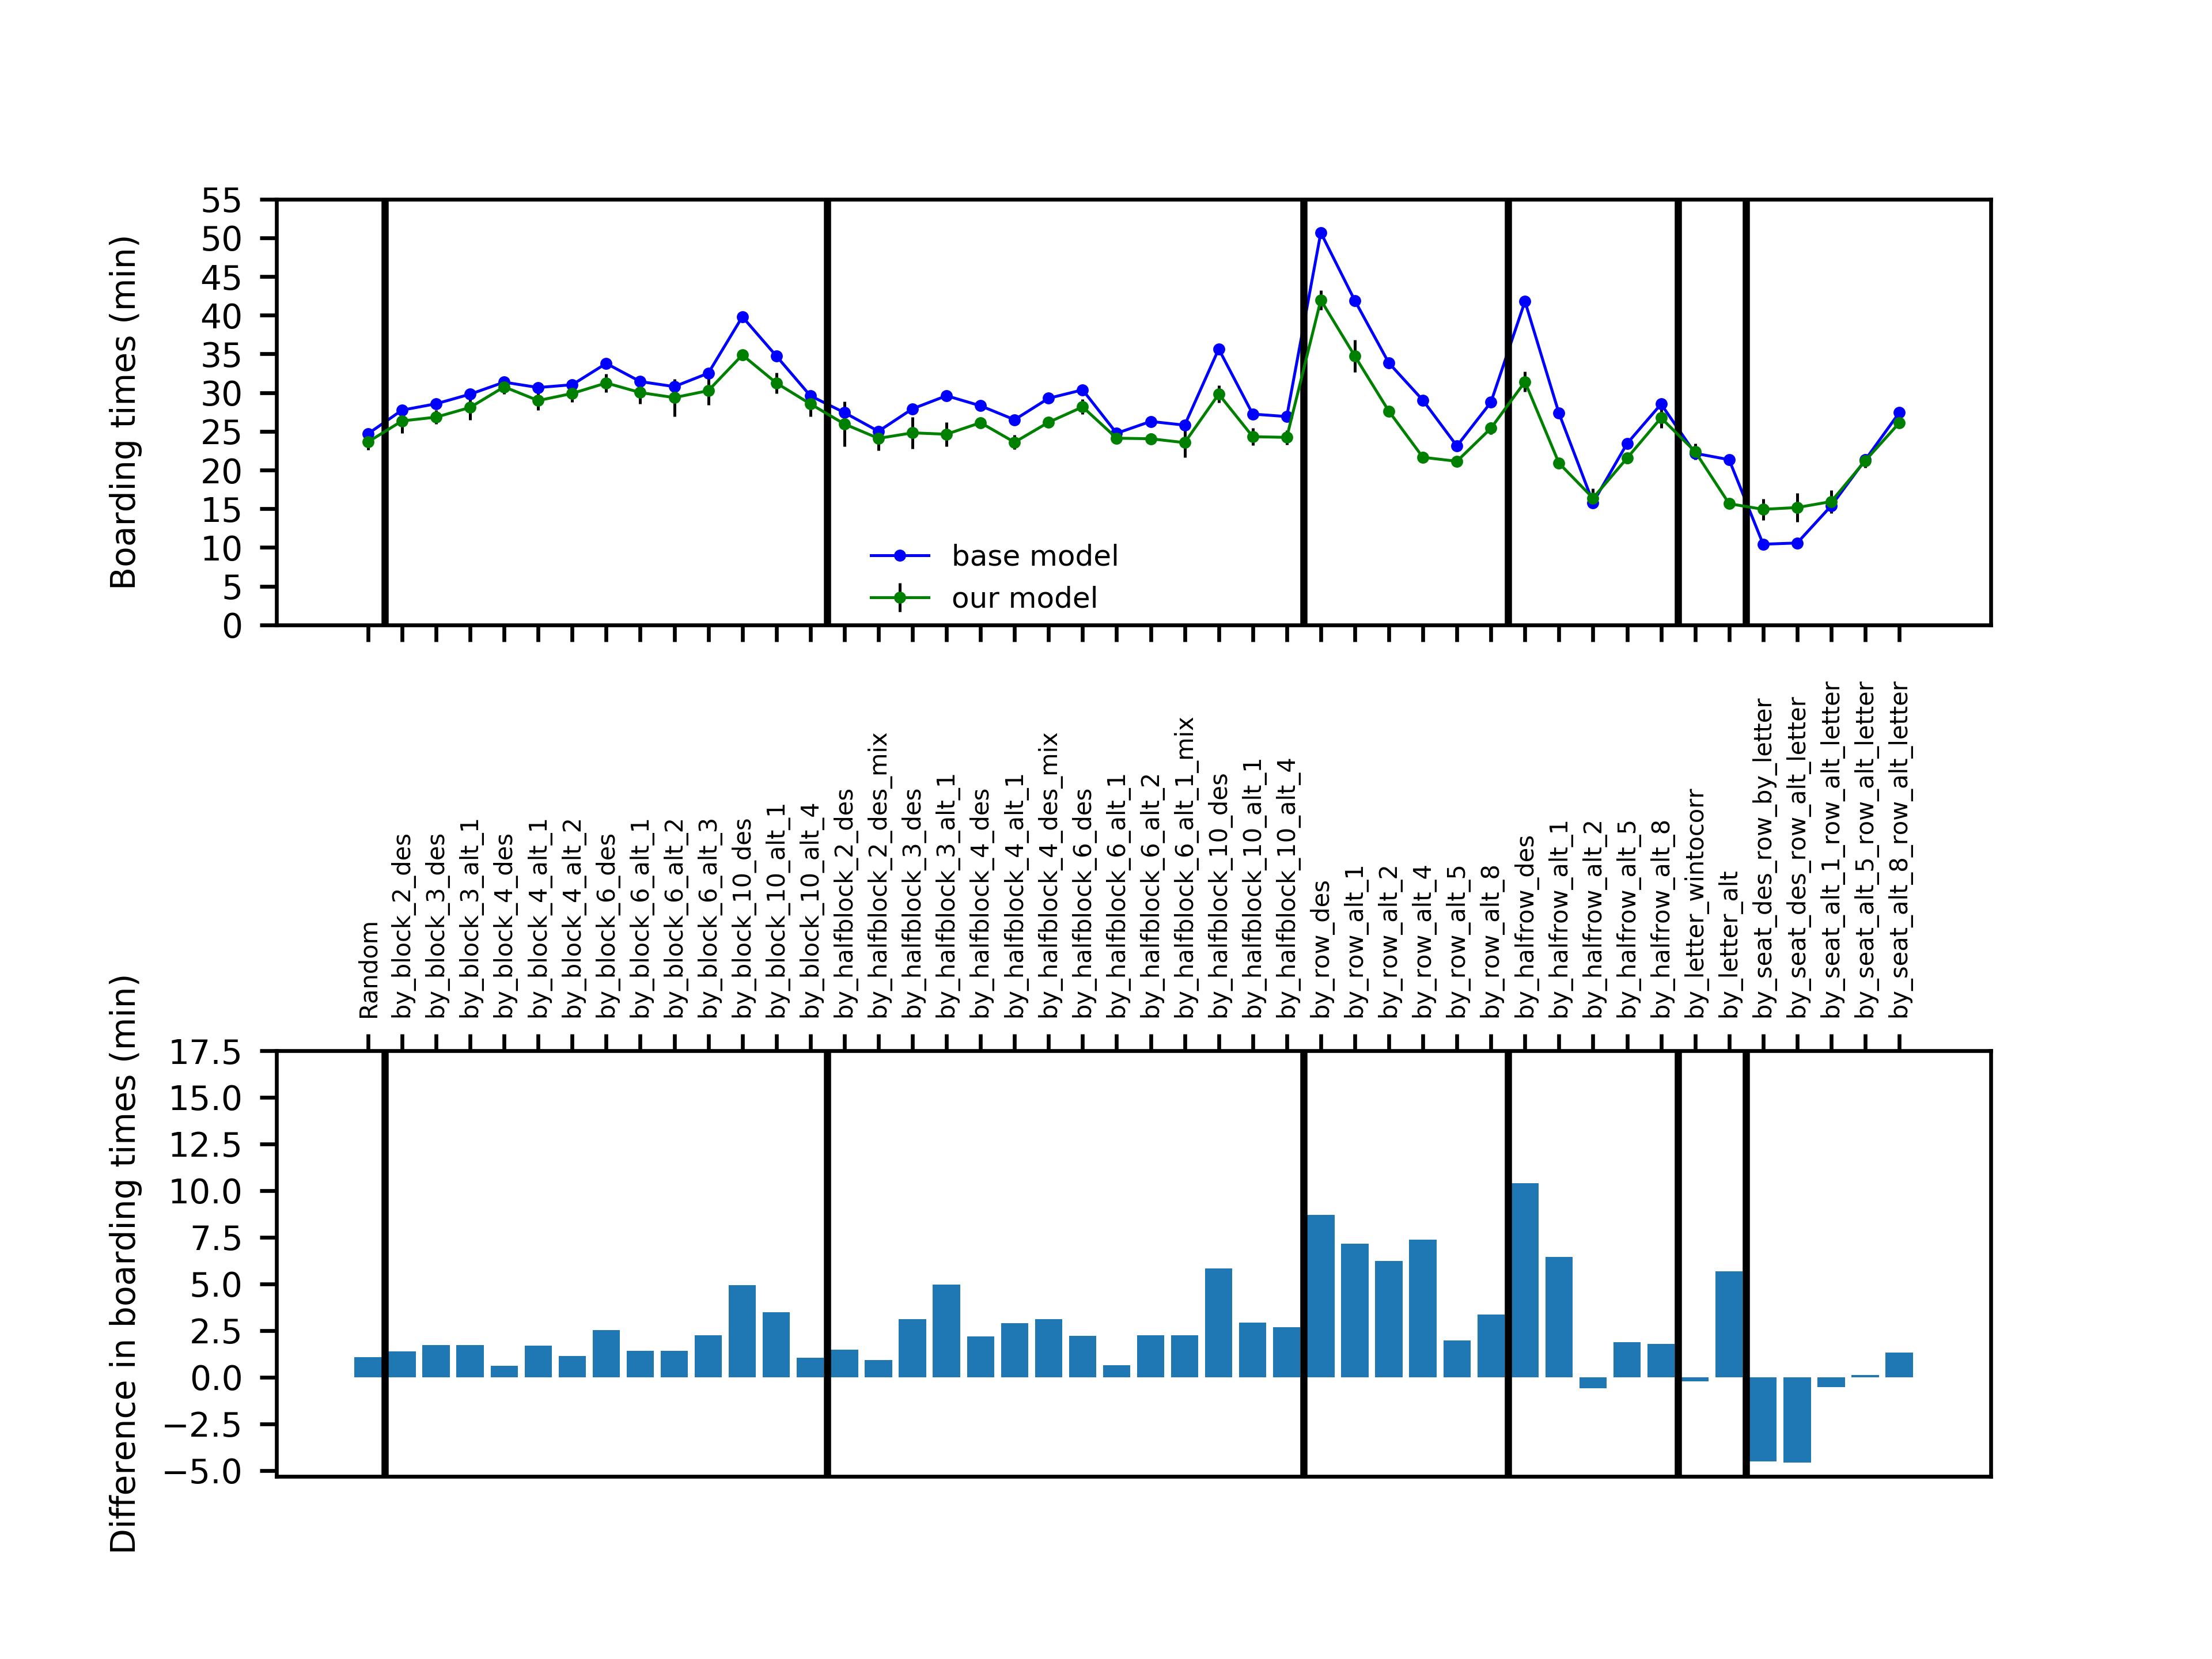
\includegraphics[width=\linewidth]{../../code/AirplaneBoarding/data/figure1/figure1.png}
	\caption{This figure compares the results from our model, using a similar airplane and load specifications, to the ones from the model used in \cite{beus}.}
	\label{figure1}
\end{figure}
\subsection{Result Comparison - Our model vs. Van Landeghem's and Beuselinck's Model}
In order to validate the correctness of our model we compare the different boarding times resulting from employing the same boarding methods as was done in \cite{beus} with a similar airplane and load level. The airplane used in both models are equivalent in the number of rows they have (23) and the number of seats in each row (6), with the only minor exception that the plane they used only had 3 seats in the first and last row. However this difference is very minor, so we decided to neglect it. The passenger load level, so the percentage of occupied seats in the aircraft, are in both cases identical at $100\%$. Furthermore the luggage load level in the simulation from Van Landeghem and Beuselinck was set to normal, which we had to translate into the percentage of occupied overhead compartment space, as our model handles luggage differently to theirs. We believe that when the plane is completely booked out, it is reasonable to assume that $90\%$ of available overhead compartment space is occupied with a normal load level.

In total for each of the 46 boarding methods (excluding method "by\_block\_B-E" because it differentiates with business class in addition to economy class, which, for given reasons, we don't do) we performed 5 trials, in order to have a small sample to calculate the mean time taken for each boarding method within a $95\%$ confidence interval.
The results for the confidence intervals of the total boarding times and differences to Van Landeghem's and Beuselinck's results (their minus our) are displayed in Figure \ref{figure1}. For numerical values, please check table \textit{Insert reference here} in the Appendix.
Analysing the results lead to following conclusions:


The first conclusion that can be drawn is that the average boarding times for our model are generally lower with only a few exceptions. This phenomenon is most likely caused by the different ways the two models handle luggage. In our model the time it takes to store luggage inside a specific compartment does not increase with the amount of luggage that is already inside, which is the case for the other model. Furthermore, not everyone necessarily has any luggage with them because the number of actors (138) is much larger than the total amount of hand-luggage (75) distributed between them (no one more than 2 pieces), which means there are plenty which can directly move to their seat. In the case of the other model, every actor has between 1 and 3 pieces of luggage, so in total almost at least twice the amount of carry-on luggage and there is no one without any. These two aspects further support the results. On the other hand, compartments can be full, not allowing any more actors to store any of his carry-on inside of it, which means those actors have to find other free spots, which takes time and can cause interferences.  To what extend each of these aspects impacts the result can not be said as we have not enough information about the model used in \cite{beus}. 
	
The two exceptions to this observations occur in the class "by\_seat", but only with the two that do not alternate between rows. The reason for that is most likely that the actors in our model first always try to store their luggage in the overhead compartment above their seat and if possible start storing at the beginning of it, not allowing the actor behind to access the same compartment. So if actors that are right behind each other in the boarding sequence have seats in the same or adjacent rows, they might obstruct one another when they both have hand-luggage. This is would also explain why the exception is only seen in the two methods within class "by\_seat" that do not alternate between rows, so adjacent actors in the boarding sequence have adjacent rows. This attribute of the actors only negatively impacted the difference in time in one class because in all the others we look at larger groups, which are random within, and not at individual seats and arrange those. Because the exception to the phenomenon, that the times of our model are generally lower, only occurs in those two methods and is caused by something reasonable, the validity of our model is not impacted. 

Now, in order to be able to conclude that our model is at least as valid as the one used by Van Landeghem's and Beuselinck's, we need to evaluate the impact that the found phenomenon has. 

First of all, the general trend of the data is retained by our model because within each class, especially the larger ones, the difference in boarding times is fairly constant, which again can be seen in the bottom diagram of Figure \ref{figure1}. 


\section{Summary and Outlook}

\section{References}
\begin{thebibliography}{9}
	\bibitem{beus}
	Van Landeghem, H, and A Beuselinck. 
	\textit{"Reducing Passenger Boarding Time in Airplanes: A Simulation Based Approach."} 
	European Journal of Operational Research, vol. 142, no. 2, 2002, pp. 294–308.,
	doi:10.1016/s0377-2217(01)00294-6.
	
	\bibitem{nasa}
	Data Passenger Size from:  NASA. “Man-Systems Integration Standards.” Man-Systems Integration Standards, vol. 1, July 1995, p. 30.
\end{thebibliography}





\end{document}  



 
